%definición del artículo
\documentclass[a4paper,12pt,openany,oneside]{book}
\usepackage[left=5cm,right=2cm,top=4cm,bottom=4cm,paperwidth=216mm,paperheight=330mm,pdftex]{geometry}
%paquete usado para silabación en español
\usepackage[spanish]{babel}
%codificación del documento
\usepackage[utf8]{inputenc}
%espaciado
\linespread{1.5}
%identación de párrafo
\setlength{\parindent}{20pt}
%espaciado de párrafo
\setlength{\parskip}{4ex plus 0.5ex minus 0.2ex}
%para validar sólo sintaxis sin compilar
%\usepackage{syntonly}
%\syntaxonly
%para usar imágenes
\usepackage{graphicx}
%para usar fragmentos de codigo fuente
\usepackage{listings}
\usepackage{float}
%para usar signos de check y wrong
\usepackage{bbding}
%para usar colores en textos y simbolos
\usepackage{color}
\usepackage{multirow} %multi columna
\floatstyle{boxed}
\newfloat{codigo}{thp}{lop}
\floatname{codigo}{Caja de Código}

%comienzo del documento
\begin{document}
%\thispagestyle{empty}

\begin{center}
\textbf{UNIVERSIDAD TECNOLÓGICA METROPOLITANA\\
FACULTAD DE INGENIERÍA\\
ESCUELA DE INFORMÁTICA}\\
\vspace{3cm}
SISTEMA INTEGRADOR Y MANTENEDOR DE DATOS EN SEPA
\end{center}
\begin{flushright}
TRABAJO DE TÍTULO PARA OPTAR AL\\
TÍTULO DE INGENIERO CIVIL EN\\
COMPUTACIÓN\\
MENCIÓN INFORMÁTICA\\
\vspace{3cm}
Sebastián Salazar Molina\\
\vspace{1.5cm}
ALUMNO: Miguel Ángel Aníbal Davor Fuenzalida Pino
\end{flushright}
\vspace{4cm}
\begin{center}
SANTIAGO - 2013
\end{center}
\newpage
\thispagestyle{empty}
\begin{flushright}
\vspace{20mm}
Nota: \line(1, 0){140} \\
\vspace{30 mm}
\line(1, 0){180}\\	
Firma y Timbre\\
Autoridad Responsable
\end{flushright}
\chapter*{Resumen}
\thispagestyle{empty}
En las organizaciones, para manipular los recursos y la toma de decisiones, es necesario el uso de información procesada, el cual entrega valor agregado.

La UTEM dispone del sistema S.E.P.A,. (Sistema Estadístico de Profesores y Alumnos), que consiste en un proyecto Web realizado en PHP que toma datos de alumnos, profesores y encargados provenientes de DirDoc, para posteriormente hacer cálculos predefinidos con el fin de mostrar indicadores que representen la realidad universitaria.

Sin embargo S.E.P.A. presenta insuficiencias: No se disponía de un servicio web (una forma de acceso mas segura y controlada) que se comunique con DirDoc; Hay inconsistencia en los datos.

% ejemplos, no tiene servicio web dirdoc, inconsistencia de datos, carece de formas alternativas de accesos, carece multiples roles (más de 2).

El presente trabajo de Título ofrece una mejora al sistema S.E.P.A., con integración de herramientas que permiten mejoras por la universidad (serán explicadas a fondo en este documento). Las herramientas usadas en este proyecto son: 

\begin{itemize}
	\item El sistema gestor de bases de datos PostgresSQL.
	\item Herramienta de construcción de proyectos MAVEN para el lenguaje de programación Java.
	\item Uso de servicios web con CXF.
\end{itemize}

\tableofcontents
%\listoffigures
\chapter*{Introducción}
\thispagestyle{empty}
La Universidad Tecnológica Metropolitana utiliza para la administración de toda la información referente a estudiantes, profesores y personal de administración un proyecto denominado Sistema Estadístico de Profesores y Alumnos (S.E.P.A.) basado en la tecnológica PHP. Este proyecto constituyó una forma de potenciar las capacidades operativas de la Universidad, generando indicadores de calidad y entregando una ventaja comparativa frente a otras universidades.

La incidencia de este trabajo de título esta en la actualización del proyecto SEPA usando la tecnología Java que utiliza herramientas más estructuradas, extensibles y que tienen como resultado la materialización de sistemas informáticos más fácilmente mantenibles debido al uso de patrones de Diseño (explicados en este informe). Por ejemplo, se utilizará el Modelo Vista Controlador o una Persistencia basada en JPA (adaptador de persistencia en java, para establecer el modelo de base de datos solo con código java), Spring (para facilitar el desarrollo de la lógica del negocio) y PrimeFaces (paquete de desarrollo que se utiliza sobre java para mostrar una visualización cómoda para los usuarios, posee varias herramientas hechas para trabajar en sitios web). 

Además, el proyecto se hará bajo la metodología PSP (Personal Software Process) que nos proporciona un modelo de trabajo basado en la caracterización de los tiempos y costes del trabajo de un ingeniero informático, adicionando documentación extra (explicada en este informe), correspondiente a eventos que caracterizaron las directrices de cómo se lleva adelante este trabajo, todo lo cual, conduce a una evaluación de la calidad del proyecto como programa.

Existen 3 tipos de beneficios que la Universidad puede obtener al hacerse con la versión mejorada del sistema SEPA:

\begin{enumerate}
\item La universidad se muestra al mercado como un ente preocupado de medir su calidad con herramientas tecnológicas que justifican un buen desempeño mediante indicadores cuantificables y verificables por 
organismos reguladores.

\item Beneficio de los usuarios, los cuales se ven favorecidos, ya que tendrán a su disposición una completa herramienta que los apoyará en la elección de su carga academia, gracias a la visualización de su desempeño posterior.

\item Beneficio a futuro, dado el alto estándar de las herramientas utilizadas, la integración, en términos de programación, debiese resultar más sencilla, ya que este proyecto esta realizado bajo tecnologías más estandarizadas como lo son los proyectos desarrollados en java, maven, spring.
\end{enumerate}

\chapter{Antecedentes}
\thispagestyle{empty}
\section{Contexto General}
Lo expuesto en este documento esta inmerso en la Universidad Tecnológica Metropolitana (UTEM), la cual es un organismo de enseñanza superior que se encuentra dentro del Consejo de Rectores de las Universidades Chilenas. Además estamos en el ámbito de la administración de la misma universidad, esto quiere decir que hablaremos sobre los manejos de información que están dentro de sistemas informáticos que posee la universidad como por ejemplo el anterior SEPA y el DirDoc.
\section{Contexto Particular}
El proyecto SEPA (Sistema Estadístico de Profesores y Alumnos, es el encargado de mostrar información que pueda ser cuantificable en pos de tener herramientas de control general y toma de decisiones. Dicha información viene del sistema DirDoc que se utiliza para la mantención de datos académicos en la universidad.
\section{Problema}
El antiguo S.E.P.A. presenta faltas o insuficiencias, tales como: 
\begin{itemize}
	\item No se disponía de un servicio web (una forma de acceso mas segura y controlada) de DirDoc.
	\item Se detectaba inconsistencia en los datos.
	\item Carecía de múltiples tipos de usuarios, diferenciando sus actividades.
	\item No existía una forma sencilla de modificar y actualizar la información.
\end{itemize} 
\section{Motivación}
Ayudar a mejorar las herramientas de administración de la Universidad y aprender a desarrollar tecnologías que apoyan a instituciones públicas, los cuales, ayudan a la gente.
Para lograr esto se completarán las siguientes tareas:
\begin{itemize}
	\item Acceder a un servicio web para obtener los datos de manera segura.
	\item Crear un mantenedor de todos los datos que podamos integrar en el servicio web.
	\item Automatizar los procesos de acceso y actualización de datos.
\end{itemize}
\chapter{La Organización de la UTEM}
\thispagestyle{empty}
\section{Misión}
La Universidad Tecnológica Metropolitana es una organización estatal enfocada en la generación de profesionales que estén a la altura de los proyectos que se necesitan en pos de mejorar el país de manera sólida, segura y tecnológica. Para este motivo transforma a personas en profesionales con altas capacidades para enfrentar problemas. Estos profesionales se caracterizan por la fuerte convicción de lograr sus objetivos incluso en situaciones difíciles.
\section{Visión}
La organización será un ente de enseñanza que contará con una inclusión de profesionales de un alto nivel académico, mejorando así su capacidad de formar a los profesionales del futuro. Tendrá áreas de investigación y creación tecnológica que permitirán la modernización en muchas áreas del conocimiento. La organización se caracterizará por la prescindencia de todo tipo de discriminación de genero, religión y raza.
%\section{Organigrama Empresarial}

\section{Estructura de desarrollo el proyecto}
El desarrollo del proyecto esta bajo la metodología Personal Sofware Process (PSP), la cual permite medir en forma cuantitativa todas la variables implicadas en el proceso productivo de este proyecto, lo que brindará valiosa información tanto del proyecto como del alumno.
\chapter{Problema}
\thispagestyle{empty}
\section{Situación Actual}
La organización dispone del sistema SEPA, el cual tiene una paleta de funcionalidades, que esperan en un futuro poder mejorar. Por ejemplo hoy se pueden generar gráficos y variables estadísticas que muestran información útil a la hora de tomar decisiones. Los profesores o funcionarios pueden entrar a mirar datos y comprobar indicadores. Para estos efectos ya se han pedido mejoras e inclusión de más actores frente a este sistema, mejorando no solo su funcionalidad si no que también agregando características de seguridad y mejora de la calidad de los datos.
\section{Situación Propuesta}
Una serie de módulos de mantenimiento de datos para arreglar los defectos que se presenten en todos los datos (provenientes del DirDoc) que son expuestos en los servicios web. Un sistema automatizado de integración con DirDoc,  para mantener actualizado Sepa, sin la necesidad de procesos manuales y directos en base de datos.
\section{Objetivos Generales y Específicos}
\subsection{Objetivos Generales}
\textit{Desarrollar un sistema de mantención de información estadística para la Universidad Tecnológica Metropolitana ayudando a sus procesos docentes y productivos, disponiendo de información veraz de la realidad universitaria.}
\begin{enumerate}
\item Crear un sistema web basado en el patrón Modelo Vista Controlador, asegurando un producto que sea eficiente en el cumplimiento de sus objetivos. Las características principales serán que este sistema estará hecho en Java lo que nos permite una fácil implementación de las mejores prácticas de programación.
\item Otro objetivo es la utilización de una metodología de desarrollo, en este caso PSP (Personal Software Process), la cual nos permite llevar un seguimiento y retroalimentación de las actividades que se deben realizar, de manera lógica y ordenada, para este propósito la metodología propone la utilización de valores contables en el tiempo, estos valores establecen las características y condiciones del trabajo del ingeniero.
\end{enumerate}
\subsection{Objetivos Específicos}
\begin{enumerate}
	\item Generar un sistema que sea fácilmente mejorable, usando tecnologías estandarizadas y óptimas.
	\item Mostrar el desarrollo del proyecto a través de la metodología PSP.
	\item Entregar un producto de calidad, escalable y fiable para la comunidad universitaria.
\end{enumerate}
%\chapter{Alcances y Limitaciones}
%\thispagestyle{empty}
%\section{Alcances del Proyecto}
%La coparticipación de indicadores UTIGRA (Unidad de Títulos y Grados) para trabajar con información pertinente a %gente que ha terminado sus procesos estudiantiles en la UTEM.

%Se crearan una serie de nuevos perfiles, y cada uno de estos tendrán su nivel de alcance en el sistema.
%\section{Limitaciones del Proyecto}
%El proyecto no contendrá requerimientos que se hagan fuera de lo requerido por el profesor como actividades de %Trabajo de Título.
%\section{Alcances del Trabajo de Título}
%Los alcances del Trabajo de Título están delimitados por las características que el trabajo de título debe tener, es %decir, que se hace un marco de trabajo, delimitado por el profesor, que comprende los tópicos a trabajar.
%\section{Limitaciones del Trabajo de Título}
%El trabajo no comprende áreas que estén fuera de los límites temporales a la toma de requerimientos, por lo cual es %necesario indicar que hay características y funcionalidades que a pesar de ser levantadas puede que no sean parte de %este trabajo de título.
\chapter{Marco Teórico}
\thispagestyle{empty}
\section{Base Conceptual}
\subsection{Establecer el problema}
En la universidad existe la necesidad de mostrar información relevante para la toma de decisiones, esta información debe ser respaldada por las grandes cantidades de registros que se guardan constantemente en el sistema DirDoc de la universidad. Para este propósito existe el Sistema Estadístico de Profesores y Alumnos (SEPA), el cual otorga indicadores que pueden ser usados para la toma de decisiones. Como la universidad ha crecido, también crece la cantidad de información y la necesidad de actualizar y modificar los datos de manera más rápida y sencilla.
\subsection{Establecer la Solución}
La solución de este proyecto es la creación de un un módulo que pueda consumir los servicios web que proveen datos que deben ser procesados y persistidos en una base de datos local. Este sistema debe validad la integridad de los datos evitando perdida de registros. Mas adelante se trabaja en un mantenedor para cada uno de estos datos que compone el sistema, en los cuales es posible buscar registros, comprobar que estén correctos, si no lo están, poder modificarlos.
\subsection{¿Por qué ocupar Java?}
El proyecto es construido a través del compendio de tecnologías que engloba la convención JEE, ya que de esta manera nos enfocamos en el proceso productivo de una manera bastante estandarizada, gracias a esta forma de trabajo podemos automatizar varios procesos y centrarnos en el proyecto.Eso facilita la construcción del proyecto de manera más flexible y rápida. Todo con el fin de realizar de la mejor manera posible este proyecto que beneficia a la universidad.
\subsection{¿Por qué no otras tecnologías?}
Otras tecnologías como PHP nos permite crear la pagina de manera rápida e incorporar un framework de persistencia. Pero son difíciles de escalar y mantener.  Otros frameworks como Ruby on Rails podría llevar a cabo esta tarea de mejor manera. Pero el punto frágil de Ruby es que su curva de aprendizaje es bastante costosa.

% enfocar a las cosas que no se pueden haceren otros lenguajes.
\section{Ciclo de vida del Software}
\begin{enumerate}
\item Toma de Requerimientos: Proceso que básicamente comprende 2 actividades, primero la toma de requerimientos en base al sistema SEPA anterior, segundo una serie de entrevistas para captar las historias de usuarios que posteriormente se convierten en requerimientos.
\item Análisis de Requerimientos: Etapa en donde el profesor encargado discute con el alumno los requerimientos deben realizarse, de acuerdo con las expectativas y las necesidades del equipo de trabajo.
\item Diseño de la solución: Proceso en donde se desarrolla el modelo de datos que debe soportar a los requerimientos, y las interfaces asociadas.
\item Diseño Estructural: En este punto el alumno trabaja desarrollando el proyecto en coordinación con el profesor encargado y este va revisando constantemente el avance, emitiendo preferencias y aclaraciones.
\item Pruebas: Proceso por el cual el sistema en una fase anterior al termino de proyecto se encuentra en estudio, el profesor encargado verifica la fiabilidad y calidad de los requerimientos ya resueltos.
\item Instalación: En este punto se produce la incorporación del sistema en su ambiente por defecto, lo que implica un termino del proyecto, solo dentro del marco de trabajo de título para el alumno de este proyecto.
\end{enumerate}
\section{Historia del Arte}
La calidad de datos que se obtienen en un establecimiento educacional, es de vital importancia para la planificación y desarrollo de sus actividades, ya que permiten una normal toma de decisiones que afectan el crecimiento de la institución, ya sea de forma docente como administrativa. 

Los estudios estadísticos son importantes por que entregan retroalimentación. Buscando como objetivo llegar más cerca de su visión como organización.

Las instituciones educacionales que producen profesionales deben estar evaluadas por organismos preparados en testificar las características de su desempeño. Para estos efectos, existen organismos estatales que acreditan lo que cada universidad propone, pero en otro lado existen entandares de calidad que son medidos por organismos extranjeros, para dar un sello de calidad, evaluado por datos estadísticos  \cite{data1}.

En 2009 se abre el sitio QS Top Universities que hasta el día de hoy es un sitio altamente eficiente en evaluación a trabes de ránkings enfocados a entregar información a gente proveniente de post-grados, MBA, estudios de ingeniería y negocios. Desarrollando estadísticas de alto alcance en sitios web, eventos, guias y programas por Internet y finalmente entregando soluciones técnicas a otros organismos, tales como universidades o empresas privadas, entre otras.

Sus datos manejan información de 41 países, entre los que están: Argentina, Ecuador, Japon, Singapur, Australia, Egipto. Su servicio esta libre para todo el publico y permite un tipo de suscripción gratuita para visualizar tablas comparativas de manera bien simple.

Permite hacer comparaciones por categorías varias, ya sea país, estado, ciudad y otras características internas de la universidad como ponderaciones o prestaciones de alumnos, tales como cantidad de alumnos o la segregación por sexo o etnia en cada localidad.

Su objetivo es ser el principal sitio de ránkings de educación con visualización con alcances estadísticos y comparativos a quienes estén dentro de su sistema.

Una debilidad de este sistema es que solo hace comparaciones de carácter global y no se involucra en temas más finos sobre cada universidad, solo tiene datos recopilados de otras investigaciones para saldar ese tema.

Es una empresa de tamaño mediano, con más de 150 empleados en oficinas de todo el mundo. También se realizan Tours en 70 ciudades en 39 países que permiten a más de 50.000 espectadores, los cuales buscan entrar a una universidad  \cite{data2}.

El Ránking de Calidad de las Universidades Chilenas, es un trabajo realizado por AméricaEconomía Intelligence en el 2010, un sitio de ránking para instituciones educacionales en Chile, que utiliza ciertos criterios, como lo son la cantidad de investigaciones, o la masa de estudiantes que entran en cada universidad.

%Algunos datos generales que se obtienen, son que la Universidad de Chile y la PUC, tienen diferencias muy pequeñas %en el campo de la investigación, para lo cual se mostró que la Universidad de Chile aporto con 1.329 papers %publicados, en cambio la PUC hizo un aporte total de 1.029 publicaciones.

Mucha de esta información estadística es recopilada a traves de encuestas enviadas a distintas universidades y organismos de educación en Chile. De esta manera se puede obtener información importante para ser mostrada al publico que desea tomar una decisión en el mercado.

Este sistema da cuenta de una necesidad por parte de las universidades, de ser más competitiva en el mercado universitario. Aumentando los esfuerzos por adquirir más estudiantes, mostrando mejores profesores, alumnos e investigaciones.

La gran debilidad de este sistema es que no se efectúan muchos criterios de comparación y por tanto solo da una arista para presentar la comparación lo que resulta incomodo al no poder ver desde otra perspectiva este sistema.

Finalmente se nota a las universidades actuales buscando organismos extranjeros capaces de certificar las características de la educación que ofrecen, de esta manera muestran no solo una acreditación por un organismo chileno, si no también una necesidad por competir a nivel internacional \cite{data3}.

\section{Justificación del Trabajo de Título}
La universidad necesita un sistema que agregue funcionalidades que son necesarias para el control de sus datos de manera simple y segura. En el anterior SEPA los datos eran extraídos directamente del DirDoc, dando la posibilidad de cometer errores de inserción graves. Con este nuevo sistema, ahora no solo hay una seguridad con los datos que son transferidos desde servicios Web, si no que también implementa un sistema de autenticación, gracias a su sistema de perfiles de usuarios que limita el acceso en el sitio para mas de 2 tipos de usuarios.

Existe una razón económica, prima por otras ya que un sistema de esta envergadura requiere no solo dinero si no también el consentimiento de varias entidades de poder dentro de la universidad, para realmente tomar la decisión de comprar un sistema externo.

Finalmente el punto negativo de todo esto, es que este trabajo esta acotado dentro de los margenes que debe tener un trabajo de Título, por lo tanto no es posible seguir en el desarrollo a menos que exista una visión de futuro y/o parte del profesor a cargo de este proyecto con el alumno que realiza este trabajo.
\section{Análisis de las herramientas}
El desarrollo de las aplicaciones debe ser con un lenguaje que nos permita la correcta ejecución de las tareas de diseño y desarrollo. Por lo cual resulta interesante desarrollar algunos criterios que nos mostrarán las características y la justificación de nuestra elección a la hora de pensar en un lenguaje apropiado para este proyecto.

\begin{enumerate}

\item Sencillez: Característica del lenguaje que hace que sea fácil el crear o entender el código, al momento de programarlo o leerlo \cite{data4}.

\item Robustez: Capacidad interna del lenguaje de proporcionar herramientas que permiten minimizar los errores producidos por el programador \cite{data4}.

\item Seguridad: Característica que hace que un lenguaje no permita tocar accesos a donde la aplicación no debiese ir (en la mayoría de los casos), ejemplos como, restringir accesos, ejecución de pruebas o derechos de accesos \cite{data4}.

\item Portabilidad: Capacidad de un lenguaje para correr en múltiples sistemas operativos \cite{data4}.

\item Neutralidad: Independencia de la maquina en donde se ejecuta, haciendo una experiencia lo más similar posible entre distintas máquinas y sistemas operativos \cite{data4}.

\item Interfaz: Capacidad de producir fácilmente interfaces cómodas para el usuario final \cite{data4}.

\item Expresividad: Cantidad de lineas con las que una acción puede ejecutarse dentro del código \cite{data5}.

\item Compilación: Se refiere al tiempo que toma poder compilar el código producido.

\item Aprendizaje: Dificultad para aprender el lenguaje. Basado simplemente en la experiencia propia sobre cada lenguaje.

\item Estructuras de control: Un lenguaje debe proveer estructuras simples de control, pero tampoco llenarse de estructuras que nunca se van a utilizar \cite{data6}.

\item Abstracción: Capacidad de convertir cosas difíciles en algo simple con la estructura del lenguaje \cite{data6}.

\end{enumerate}

También es importante tener en cuenta el lenguaje a utilizar en el momento de la creación del proyecto, de esta manera se pondrán los lenguajes candidatos para conocerlos en mayor detalle.

\begin{enumerate}

\item PHP: Es el lenguaje de lado servidor más extendido en la web. Surgido en 1994, se trata de un lenguaje de creación relativamente reciente, aunque con la rapidez con la que evoluciona Internet parezca que ha existido toda la vida. Es un lenguaje que ha tenido una gran aceptación en la comunidad de desarrolladores, debido a la potencia y simplicidad que lo caracterizan, así como al soporte generalizado en la mayoría de los servidores \cite{data7}.

\item .NET: Es un framework de Microsoft que hace un énfasis en la transparencia de redes, con independencia de plataforma de hardware y que permita un rápido desarrollo de aplicaciones. Basado en ella, la empresa intenta desarrollar una estrategia horizontal que integre todos sus productos, desde el sistema operativo hasta las herramientas de mercado \cite{data8}.

\item Ruby on Rails: Es un entorno de desarrollo web de código abierto que está optimizado para satisfacción de los programadores y de la productividad. Te permite escribir un buen código favoreciendo la convención antes que la configuración \cite{data9}.

\item Java: Es un lenguaje de programación con el que podemos realizar cualquier tipo de programa. En la actualidad es un lenguaje muy extendido y cada vez cobra más importancia tanto en el ámbito de Internet como en la informática en general. Está desarrollado por la compañía Sun Microsystems con gran dedicación y siempre enfocado a cubrir las necesidades tecnológicas más punteras \cite{data10}. 
\end{enumerate}

En la siguiente tabla muestra una comparación de las cuatro tecnologías anteriormente presentadas de forma explicita para comprender nuestra elección. Es claro decir que uno de los aspectos que marca profundamente la elección sobre el lenguaje con que se va a realizar este proyecto, es determinada por los conocimientos que tiene el alumno y las indicaciones del profesor, en pos de realizar lo más rápido posible el trabajo, haciéndolo de forma elegante. 

\begin{tabular}{| l | l | l | l | l |}
\hline
 & 
\includegraphics[scale=0.08]{images/icons/php.png} & 
\includegraphics[scale=0.08]{images/icons/net.png} & 
\includegraphics[scale=0.51]{images/icons/ruby-on-rails.png} & 
\includegraphics[scale=0.1]{images/icons/java.png}\\
\hline
\textit{Sencillez} & \textcolor{green}{\CheckmarkBold} &  \textcolor{red}{\XSolidBold} &  \textcolor{red}{\XSolidBold} & \textcolor{green}{\CheckmarkBold}\\
\hline
\textit{Robustez} & \textcolor{red}{\XSolidBold} & \textcolor{green}{\CheckmarkBold} & \textcolor{green}{\CheckmarkBold} & \textcolor{green}{\CheckmarkBold}\\
\hline
\textit{Seguridad} & \textcolor{red}{\XSolidBold} & \textcolor{red}{\XSolidBold} & \textcolor{green}{\CheckmarkBold} & \textcolor{green}{\CheckmarkBold}\\
\hline
\textit{Portabilidad} & \textcolor{green}{\CheckmarkBold} & \textcolor{red}{\XSolidBold} & \textcolor{red}{\XSolidBold} & \textcolor{green}{\CheckmarkBold}\\
\hline
\textit{Neutralidad} & \textcolor{green}{\CheckmarkBold} & \textcolor{red}{\XSolidBold} & \textcolor{green}{\CheckmarkBold} & \textcolor{green}{\CheckmarkBold}\\
\hline
\textit{Interfaz} & \textcolor{red}{\XSolidBold} & \textcolor{green}{\CheckmarkBold} & \textcolor{green}{\CheckmarkBold} & \textcolor{green}{\CheckmarkBold}\\
\hline
\textit{Expresividad} & \textcolor{green}{\CheckmarkBold} & \textcolor{red}{\XSolidBold} & \textcolor{green}{\CheckmarkBold} & \textcolor{red}{\XSolidBold}\\
\hline
\textit{Compilación} & \textcolor{green}{\CheckmarkBold} & \textcolor{red}{\XSolidBold} & \textcolor{green}{\CheckmarkBold} & \textcolor{red}{\XSolidBold}\\
\hline
\textit{Aprendizaje} & \textcolor{green}{\CheckmarkBold} & \textcolor{red}{\XSolidBold} & \textcolor{green}{\CheckmarkBold} & \textcolor{green}{\CheckmarkBold}\\
\hline
\textit{E. de control} & \textcolor{green}{\CheckmarkBold} & \textcolor{green}{\CheckmarkBold} & \textcolor{green}{\CheckmarkBold} & \textcolor{green}{\CheckmarkBold}\\
\hline
\textit{Abstracción} & \textcolor{green}{\CheckmarkBold} & \textcolor{red}{\XSolidBold} & \textcolor{red}{\XSolidBold} & \textcolor{green}{\CheckmarkBold}\\
\hline
\textbf{Total} & 8 & 3 & 8 & 9\\
\hline
\end{tabular}

Como lo muestra la tabla anterior, java es el que puede cumplir más criterios, en el sentido de la observación y el criterio subjetivo del alumno que realiza el trabajo.

\section{Criterios de Calidad}

Se mostrarán a continuación los criterios de calidad que el proyecto como tal va a proporcionar a la universidad. Estos criterios muestran de forma justificada, que la mejor elección es la que nosotros proponemos para la organización, pensando en los costes de tiempo y recursos económicos que un proyecto de esta clase puede significar.

\begin{enumerate}

\item Mantenibilidad: Característica que hace que nuestro proyecto sea fácil de corregir en caso de fallos, mas que nada se refiere a si las bases de nuestro proyecto están debidamente revisadas. Basándose en la concepción de que un proyecto que tiene un modelo bien establecido es más fácil de reparar \cite{data11}.

\item Flexibilidad: Característica que permite a nuestro proyecto un fácil modelo de cambios o adiciones de más características, incluyendo también el echo de que como es un sistema echo dentro del contexto de la Universidad esta lo suficientemente enfocado en ella, pero también es posible cambiar algunas cosas en pos de que este sistema funcione también en otras universidades. \cite{data11}.

\item Testeabilidad: Esto nos muestra que el modelo del sistema ha pasado por un test antes de ser ocupado en el proyecto, de manera tal como es. \cite{data11}.

\item Portabilidad: Ya que como se trabaja con Java, el proyecto es básicamente portable a casi cualquier tipo de sistema operativo, lo que lo hace un ente fácil de cambiar en otros entornos de trabajo y es perfectamente acomodable en ese sentido. \cite{data11}.

\item Integridad: Este sistema se caracteriza por su integridad con los datos, lo que nos muestra un dedicado trabajo sobre el tema de la base de datos. \cite{data11}.

\item Rapidez: El sistema esta echo de tal manera que debe funcionar de forma expedita y veloz, sobretodo con la enorme cantidad de datos que se van a manejar. \cite{data11}.

\end{enumerate}

\section{Patrones de Diseño}
Son arquitecturas estandarizadas para del desarrollo de software, permiten a los proyectos ser resueltos con estrategias ya probadas y que funcionan en la mayoría de los casos. Existen muchos patrones distintos, algunos de ellos son:

\begin{enumerate}

\item MVC, Modelo Vista Controlador: Establece que el software tiene por lo menos 3 capas de desarrollo las cuales son; modelo, donde se encuentran el acceso a datos como de una base de datos, ficheros o servicio web; vista, la parte del programa que interactúa con el usuario final; controlador, el código en donde esta el negocio que procesa los datos del modelo para posteriormente mostrarlos en la vista.

\item SOA, Arquitectura orientada a servicios: Establece el software enfocado a los procesos de negocio, teniendo distintas capas de aplicaciones como: Aplicaciones básicas, caracterizadas por ser pequeñas y geográficamente establecidas; Exposición de Funcionalidades, donde rigen servicios; Integración de servicios, para intercambio de datos; Composición de procesos, determina términos de negocio y funcionalidades; Entrega, para usuarios finales.

\end{enumerate}

\chapter{Introducción al PSP}
\thispagestyle{empty}
\section{Base Teórica}
PSP (Proceso de Software Personal) es una metodología de desarrollo para proyectos informáticos, que tiene una serie de pasos enfocados en el ordenamiento, cuantificación y la categorización del trabajo y el tiempo. Es usada mundialmente por su fácil aprendizaje y su rápida incorporación. Este modelo de trabajo es solo para proyectos personales, osea en donde el desarrollador toma todo el trabajo por si solo.

Este tipo de trabajo nos proporciona una serie de tablas que muestran nuestros tiempos de desarrollo y avance del proyecto, básicamente en el PSP nosotros podemos obtener los tiempos de desarrollo y la cantidad de lineas de código para cada actividad o conjunto de actividades. De esta manera uno puede llegar a determinar un factor de calidad dentro de nuestro trabajo dentro de los estándares que uno estime conveniente utilizar.

PSP nos obliga a desarrollar una forma de trabajo en la cual un desarrollador programa y anota los tiempos de desarrollo y la cantidad de código que uno ha producido, dentro de distintas tablas hechas para ese propósito.

\section{Criterios para uso de PSP}
La necesidad de usar PSP fue concebida para generar un proyecto que tuviera un criterio de calidad cuantificable. Ya que nos proporcionaba tablas e indicadores que establecían con el tiempo en minutos, la cantidad de esfuerzo y errores que uno puede cometer en el trascurso del proyecto.

\section{Estructura del PSP}
\subsection{El Trabajo del Ingeniero de Sofware}
En este apartado se requiere desarrollar un lista de actividades que contemplan el desarrollo del proyecto, incluyendo todo lo que pueda servir como avances en el proyecto, ya sea investigar, reunirse con otros o desarrollar.
\subsection{La Gestión del Tiempo}
Para este punto solo se necesita la estructuración del tiempo que uno tiene sobre el tiempo que se pretende dar al proyecto. Basándose en la lista de actividades.
\subsection{El Control del Tiempo}
Para este apartado se desarrolla una tabla que contiene una lista de actividades con los tiempos de inicio y termino de cada una de las cosas que se hacen. También se anotan los tiempos perdidos, el tipo de actividad y si esta completado o no.
\subsection{Planificación de Períodos y Productos}
Este apartado se preocupa de la planificación semanal del tiempo, en la parte de desarrollo se tienen 3 tablas que nos permiten llevar los registros totales de tiempo en minutos de las actividades que hago durante la semana. La primera tabla muestra las sumas de los tiempos, la segunda muestra la actividad de las semanas pasadas y la tercera muestra el total de las semanas hasta hoy en día.
\subsection{La Planificación del Producto}
El desarrollo del proyecto requiere de un cuaderno que registre la actividad en función de los trabajos que se van realizando, para lo cual se tiene un cuaderno de trabajos que registra las actividades con sus respectivas estimaciones de tiempo, sacadas de datos anteriores. Recordar que en esta tabla se anotan los trabajos que son las actividades diarias, así que se anota uno al día.
\subsection{El Tamaño del Producto}
Para estimar los costes de tiempo y valor de cada actividad que representa parte del desarrollo del un producto como tal, es necesario establecer formas de medición para valores que pueden ser cuantificables en unidades de trabajo. Para lo cual en esta actividad de mostrarán Estimaciones de tamaños para las actividades particulares de este proyecto.
\subsection{La Gestión del Tiempo}
Para poder desarrollar las actividades, se necesita tiempo, por lo cual resulta importante el manejarlo apropiadamente, para esto se hace una estimación aproximada del tiempo que consumirá la ejecución de las actividades relacionadas con el desarrollo del trabajo que esta en curso. Se expondrán dos tablas y un marco de referencias para las aproximaciones futuras.
\subsection{La Gestión de los Compromisos}
Los compromisos que uno hace con las personas a las cuales espera entregar un proyecto, deben ser documentados, mostrando el tipo de actividad a realizar, el día, los participantes de ese compromiso, la hora en que se realiza, la fecha y finalmente lo que se recibe a cambio de la finalización de estas tareas. Es importante destacar que una correcta forma de manejar los compromisos lleva a un buen plan de trabajo.
\subsection{La Gestión de las Programaciones}
En un proyecto siempre es necesario definir las características importantes que comprenden la ejecución de cada una de las actividades que se están desarrollando, por tanto en este proyecto se tiene un registro de los puntos de control, los cuales representan las características importantes que el desarrollo de este trabajo debe comprender.
\subsection{El Plan del Proyecto}
Para generar un plan del proyecto se necesita tener un resumen de las características de como se desarrolla el trabajo, para lo cual se expondrá un molde para generar planes de proyectos, los cuales estiman la cantidad de trabajo que uno puede desarrollar de acuerdo a los trabajos anteriores que ha realizado. Finalmente se mostrará un ejemplo de estimación del tamaño del programa.
\subsection{Defectos}
El registro de los defectos es altamente importante, ya que nos permite la correcta verificación de cada incidente ocurrido dentro del proceso de desarrollo del software. El cuaderno de registro de errores se ocupa en el desarrollo de aplicaciones, y nos permite anotar un error cuando ha salido en modo de compilación para lo cual uno registra el tipo de error y el tiempo dedicado a la reparación de este error. El objetivo de esta tabla es impedir la repetición de ciertos errores que pueden ser reparados mediante del aprendizaje.\\
\\
\textbf{Tipos de Defectos}\\
\begin{tabular}{| l | l | l | l |}
\hline
10 & Documentación         & 60 & Comprobación\\
\hline
20 & Sintaxis              & 70 & Datos\\
\hline
30 & Construcción Paquetes & 80 & Función\\
\hline
40 & Asignación            & 90 & Sistema\\
\hline
50 & Interfaz              & 100 & Entorno\\
\hline
\end{tabular}

\chapter{Aplicación del PSP}
\thispagestyle{empty}
\section{Explicación}
Se mostrará la forma de desarrollo de las tablas PSP más importantes en el proyecto. Dando muestra de como es el trabajo del PSP dentro de nuestro proyecto SEPA. Tendremos el desarrollo de las tablas más importantes en el PSP frente a nuestro trabajo. Obtendremos una mirada clara frente a que es el PSP y como este permite complementar calidad en nuestro trabajo.
\section{Desarrollo del PSP}
\subsection{El Trabajo del Ingeniero de Sofware}
En estos efectos se desarrollo la siguiente tabla de actividades, con su frecuencia semanal y sus minutos.

\begin{tabular}{|l | l | l |}
\hline
\textbf{Tarea} & \textbf{Frecuencia (semanal)} & \textbf{Tiempo (minutos)} \\
\hline
Estudiar documentos & todos & 840/semana\\
\hline
Desarrollo & todos & 1260\\
\hline
Programar & todos & 2520\\
\hline
Reuniones & L, M, J & 420/semana\\
\hline
Reparar Documentos & Mi, V & 840/semana\\
\hline
\end{tabular}
\subsection{La Gestión del Tiempo}
Para este caso en particular uno puede ver que se tienen todos los días de la semana destinados para el propósito de desarrollar el proyecto ya sea en informes o programar. En menos tiempo se reparten las tareas de investigar y reparar cosas.
\subsection{El Control del Tiempo}
Se muestra la siguiente tabla de control de Tiempo, de forma resumida, para un día en especifico.

\begin{tabbing}
Estudiante: \= Miguel Angel Fuenzaldia Pino \= Fecha: \= 9/10/2012\\
Profesor: \> Sebastián Salazar Molina \>   \>  \\
\end{tabbing}
\begin{tabular}{| l | l | l | l | l | l | l | l | l |}
\hline
\textbf{Fecha} & \textbf{Comienzo} & \textbf{Fin} & \textbf{Delta} & \textbf{Actividad} & \textbf{Comentarios}\\
\hline
19/11 & 10:56 & 11:17 & 20 & Desarrollo & notebook\\
\hline
      & 11:18 & 11:35 & 15 & lectura & psp\\
\hline
      & 11:35 & 12:29 & 50 & Desarrollo & notebook\\
\hline
      & 12:30 & 12:56 & 30 & lectura & psp\\
\hline
      & 12:57 & 13:02 & 5 & Desarrollo & notebook\\
\hline
      & 13:02 & 13:29 & 30 & Almorzar & olgura\\
\hline
      & 13:30 & 15:21 & 120 & Desarrollo & notebook\\
\hline
      & 15:22 & 16:12 & 45 & lectura & psp\\
\hline
      & 15:22 & 16:00 & 40 & Desarrollo & notebook\\
\hline   
20/11 & 16:00 & 17:00 & 60 & Desarrollo & notebook\\
\hline
      & 17:00 & 18:26 & 90 & lectura & psp\\
\hline
      & 18:30 & 19:00 & 30 & Desarrollo & notebook\\
\hline 
21/11 & 18:00 & 18:30 & 30 & lectura & psp\\
\hline
      & 18:30 & 19:00 & 30 & Desarrollo & notebook\\
\hline 
26/11 & 15:00 & ... & ... & Desarrollo & notebook\\
\hline
\end{tabular}
\subsection{Planificación de Períodos y Productos}
Se muestran las siguientes tablas de planificación, de forma resumida, para comprender como se utilizan.

\textbf{Estudiante}: Miguel Angel Fuenzaldia Pino     \textbf{Fecha}: 9/10/2012\\
\begin{tabular}{| l | l | l | l | l | l |}
\hline
\textbf{Tarea} & \textbf{Reunion} & \textbf{Codificar} & \textbf{Escribir} & \textbf{Leer} & \textbf{Total} \\
\hline
\textbf{Fecha} &                  & \textbf{Programas} & \textbf{Textos} & \textbf{textos} & \\
\hline
D 18/11 & & & & & \\
\hline
L & & 180 & 60 & 60 & 350\\
\hline
M & & & & & \\
\hline
Mi & & 180 & 60 & 60 & 350\\
\hline
J & 120 & & & & 120\\
\hline
V & & 180 & 60 & 60 & 350\\
\hline
S & & & & & \\
\hline
\textbf{Totales} & 120 & 540 & 180 & 180 & 1170\\
\hline
\end{tabular}
\\
Tiempos y Medias del Período, Número de Semanas (número anterior +1): 1\\
Resumen de las semanas anteriores:\\
\begin{tabular}{| l | l | l | l | l | l |}
\hline
\textbf{Total} & 1170 & 1290 & 1170 & 1150 & 1170 \\
\hline
\textbf{Med.} & 1000 & 900 & 500 & 1000 & 1000 \\
\hline
\textbf{Máx} & 1170 & 1290 & 1170 & 1150 & 1170 \\
\hline
\textbf{Mín} & 900 & 800 & 400 & 900 & 800 \\
\hline
\end{tabular}
\\
Resumen de las semanas totales (anteriores mas última)\\
\begin{tabular}{| l | l | l | l | l | l |}
\hline
\textbf{Total} & 1170 & 2460 & 3630 & 4780 & 5950 \\
\hline
\textbf{Med.} & 1000 & 1900 & 2400 & 3400 & 4400 \\
\hline
\textbf{Máx} & 1170 & 2460 & 3630 & 4780 & 5950 \\
\hline
\textbf{Mín} & 900 & 1700 & 2100 & 3000 & 3800 \\
\hline
\end{tabular}
\subsection{La Planificación del Producto}
La siguiente tabla muestra una forma de planificación.

\textbf{Estudiante}: Miguel Angel Fuenzaldia Pino     \textbf{Fecha}: 9/10/2012\\
\begin{tabular}{|c|c|c|c|c|c|c|c|c|c|c|c|c|}
\hline
\textbf{Trab} & \textbf{Fecha} & \textbf{Pro} & \multicolumn{2}{|c|}{\textbf{Estimado}} & \multicolumn{3}{|c|}{\textbf{Real}} & \multicolumn{5}{|c|}{\textbf{Hasta la Fecha}} \\
\hline
 & & & \textbf{Tie} & \textbf{Uni} & \textbf{Tie} & \textbf{Uni} & \textbf{Vel} & \textbf{Tie} & \textbf{Uni} & \textbf{Vel} & \textbf{Máx} & \textbf{Mín} \\
\hline
\multirow{2}{*}{1} & 19/11 & Escr. & 420 & 1 & 300 & 2 & 150 & 300 & 2 & 150 & 150 & 150 \\
\cline{2-13} & \multicolumn{12}{|l|}{\textbf{Descripción:} Escribir el Engineer Notebook para los capitulos 5 al 12}\\
\hline
\multirow{2}{*}{2} & 20/11 & Escr. & 420 & 1 & 300 & 2 & 150 & 300 & 2 & 150 & 150 & 150 \\
\cline{2-13} & \multicolumn{12}{|l|}{\textbf{Descripción:} Escribir el Engineer Notebook para los capitulos 7 al 16}\\
\hline
\multirow{2}{*}{n} & & & & & & & & & & & & \\
\cline{2-13} & \multicolumn{12}{|l|}{\textbf{Descripción:}}\\
\hline
\end{tabular}
\subsection{El Tamaño del Producto}
Se tiene una muestra de tablas por actividad para determinar la cantidad total de trabajo que se realiza con respecto a lo que se tiene que tener al final.

\begin{tabbing}
\textbf{Estudiante:} \= Miguel Angel Fuenzaldia Pino \= \textbf{Fecha:} \= 19/11/2012\\
\textbf{Profesor:} \> Sebastián Salazar Molina \> \textbf{Tiempos de Actividad} \>  \\
\end{tabbing}
\textbf{Reunión}\\
\begin{tabular}{| l | l | l | l |}
\hline
\textbf{Persona} & \textbf{Tiempo} & \textbf{Temas} & \textbf{Tiempo x Tema}\\
\hline
Sebastián Salazar & 60 & 4 & 15\\
\hline
\textbf{Totales} & 60 & 4 & 15 \\
\hline
\textbf{Medias} & 60 & 4 & 15 \\
\hline
\end{tabular}
\\\\
\textbf{Lectura}\\
\begin{tabular}{| l | l | l | l |}
\hline
\textbf{Capítulo} & \textbf{Tiempo} & \textbf{Páginas} & \textbf{Tiempo x Página}\\
\hline
1-5   & 180 & 50 & 3,6 \\
\hline
6-10  & & & \\
\hline
11-15 & & & \\
\hline
16-20 & & & \\
\hline
\textbf{Totales} & 180 & 50 & 3,6 \\
\hline
\textbf{Medias} & 180 & 50 & 3,6 \\
\hline
\end{tabular}
\\\\
\textbf{Escribir}\\
\begin{tabular}{| l | l | l | l |}
\hline
\textbf{Documento} & \textbf{Tiempo} & \textbf{Páginas} & \textbf{Tiempo x Página}\\
\hline
PSP & 360 & 30 & 20 \\
\hline
Bitácora & 10 & 1 & 10 \\
\hline
Título & & & \\
\hline
\textbf{Totales} & 370 & 31 & 30 \\
\hline
\textbf{Medias} & 185 & 15,5 & 15 \\
\hline
\end{tabular}
\\\\
\textbf{Programar}\\
\begin{tabular}{| l | l | l | l | l | l | l |}
\hline
\textbf{Programa} & \textbf{LOC} & \textbf{Func. Anteriores} & \textbf{Func. Hasta} & \textbf{Mín} & \textbf{Media} & \textbf{Máx}\\
\hline
Modelo & 			500  & 400 & 200 & 200 & 400 & 500 \\
\hline
Control &			100  & 50  & 25  & 25  & 50  & 100 \\
\hline
Vista &  			400  & 350 & 175 & 175 & 350 & 400\\
\hline
\textbf{Totales} &	1000 & 800 & 200 & 200 & 800 & 1000 \\
\hline
\textbf{Medias} & 	500	 & 400 & 100 & 100 & 400 & 500\\
\hline
\end{tabular}
\subsection{La Gestión del Tiempo}
Se muestran las tablas de gestión del tiempo por actividades.

\begin{tabbing}
\textbf{Estudiante:} \= Miguel Angel Fuenzaldia Pino \= \textbf{Fecha:} \= 19/11/2012\\
\textbf{Profesor:} \> Sebastián Salazar Molina \> \textbf{Tiempos de Actividad} \>  \\
\end{tabbing}
\textbf{Toma de Requerimientos y Preparación de Engineer Notebook}\\
\begin{tabular}{| l | l | l | l | l | l |}
\hline
\textbf{Tarea} & \textbf{Reunion} & \textbf{Codificar} & \textbf{Escribir} & \textbf{Leer} & \textbf{Total} \\
\hline
\textbf{Fecha} &                  & \textbf{Programas} & \textbf{Textos} & \textbf{textos} & \\
\hline
D  &    & & 180 & 180 & 360 \\
\hline
L  & 60 & & 180 & 180 & 420 \\
\hline
M  &    & & 180 & 180 & 360 \\
\hline
Mi & 60 & & 180 & 180 & 420 \\
\hline
J  &    & & 180 & 180 & 360 \\
\hline
V  & 60 & & 180 & 180 & 420 \\
\hline
S  &    & & 180 & 180 & 360 \\
\hline
\textbf{Totales} & 180 & & 1260 & 1260 & 1440 \\
\hline
\end{tabular}
\\\\
\textbf{Etapa de desarrollo de Proyecto e Informe}\\
\begin{tabular}{| l | l | l | l | l | l |}
\hline
\textbf{Tarea} & \textbf{Reunion} & \textbf{Codificar} & \textbf{Escribir} & \textbf{Leer} & \textbf{Total} \\
\hline
\textbf{Fecha} &                  & \textbf{Programas} & \textbf{Textos} & \textbf{textos} & \\
\hline
D  &    & 180 & 180 &  & 360 \\
\hline
L  & 60 & 180 & 180 &  & 420 \\
\hline
M  &    & 180 & 180 &  & 360 \\
\hline
Mi & 60 & 180 & 180 &  & 420 \\
\hline
J  &    & 180 & 180 &  & 360 \\
\hline
V  & 60 & 180 & 180 &  & 420 \\
\hline
S  &    & 180 & 180 &  & 360 \\
\hline
\textbf{Totales} & 180 & 1260 & 1260 &  & 2700 \\
\hline
\end{tabular}
\subsection{La Gestión de los Compromisos}
La siguiente tabla muestra un ejemplo de los compromisos y la información de acuerdo a cada tarea que uno pretende realizar.

\begin{tabbing}
\textbf{Estudiante:} \= Miguel Angel Fuenzaldia Pino \= \textbf{Fecha:} \= 19/11/2012\\
\textbf{Profesor:} \> Sebastián Salazar Molina \> \textbf{Tiempos de Actividad} \>  \\
\end{tabbing}
\textbf{Lista de Compromisos}\\
\begin{tabular}{| l | l | l | l | l | l |}
\hline
\textbf{Fecha} & \textbf{Compromizo} & \textbf{¿Con quíen?} & \textbf{Horas} & \textbf{Fin} & \textbf{Consigo} \\
\hline
D  & Leer       & Propio   & 3 & Dom & Conocimiento \\
\hline
L  & Desarrollo & Cliente  & 3 & ... & Título \\
\hline
M  & Escribir   & Profesor & 3 & ... & Título \\
\hline
Mi & Desarrollo & Cliente  & 3 & ... & Título \\
\hline
J  & Reunión    & Profesor & 1 & ... & Información \\
\hline
V  & Desarrollo & Cliente  & 3 & ... & Título \\
\hline
S  & Escribir   & Profesor & 3 & ... & Título \\
\hline
\end{tabular}
\subsection{La Gestión de las Programaciones}
A continuación una tabla que muestra un poco de como una persona que utiliza el PSP puede programar su lista de actividades.

\textbf{Estudiante}: Miguel Angel Fuenzaldia Pino     \textbf{Fecha}: 9/10/2012\\\\\
\begin{tabular}{| l | l |}
\hline
\multicolumn{2}{|c|}{\textbf{Puntos de Control}}\\
\hline
\textbf{Numero} & \textbf{Punto de Control}\\
\hline
1 & Desarrollar el Cuaderno de Anotaciones para la Metodología PSP \\
\hline
2 & Asistir a reuniones con el profesor encargado del ramo \\
\hline
3 & Desarrollar el Sofware que se pide, a traves de los requerimientos conseguidos \\
\hline
4 & Escribir un informe de Título en coordinación con lo requerido\\
\hline
\end{tabular}
\subsection{El Plan del Proyecto}
Se tiene un molde de lo que es el plan del proyecto, que es la parte mas fuerte del desarrollo en PSP, ya que nos muestra información acerca de tiempos por lineas de código en un compendio de actividades que puede ser una tarea a realizar semanalmente o en periodos más largos.
\\\\
\textbf{Resumen del plan de Proyecto}\\
\begin{tabular}{| l | l | l | l |}
\hline
\textbf{Estudiante:} & Miguel Angel Fuenzaldia Pino & \textbf{Fecha:} & 19/11/2012\\
\hline
\textbf{Programa:} & Sistema mantenedor e Integrador & \textbf{Programa No.:} & 5\\
\hline
\textbf{Profesor:} & Sebastián Salazar Molina & \textbf{Lenguaje} & Java  \\
\hline
\end{tabular}
\\\\\\
\begin{tabular}{| l | l | l | l | l | l |}
\hline
\textbf{Resumen} & \textbf{Plan} & \multicolumn{2}{|c|}{\textbf{Real}} & \multicolumn{2}{|c|}{\textbf{Hasta la Fecha}} \\
\hline
\textit{Minutos/LOC} & 0.5 & \multicolumn{2}{|c|}{\textbf{1}} & \multicolumn{2}{|c|}{\textbf{180}} \\
\hline
\textit{LOC/Hora} & 120 & \multicolumn{2}{|c|}{\textbf{40}} & \multicolumn{2}{|c|}{\textbf{250}} \\
\hline
\textit{Defectos/KLOC} & 4 & \multicolumn{2}{|c|}{\textbf{10}} & \multicolumn{2}{|c|}{\textbf{50}} \\
\hline
\textit{Rendimiento} & 0.5 & \multicolumn{2}{|c|}{\textbf{0.4}} & \multicolumn{2}{|c|}{\textbf{0.45}} \\
\hline
\textit{VIF} & 2 & \multicolumn{2}{|c|}{\textbf{}} & \multicolumn{2}{|c|}{\textbf{}} \\
\hline
\textbf{Tamaño(LOC)} & \multicolumn{5}{|c|}{\textbf{2500}}\\
\hline
\textit{Nuevo y Cambiado} & 500 & \multicolumn{2}{|c|}{\textbf{300}} & \multicolumn{2}{|c|}{\textbf{1000}} \\
\hline
\textit{Máx} & 1000 & \multicolumn{4}{|c|}{\textbf{}}\\
\hline
\textit{Mín} & 500  & \multicolumn{4}{|c|}{\textbf{}}\\
\hline
\textbf{Fase(Mín)} & \textbf{Plan} & \textbf{Real} & \textbf{Hasta la Fecha} & \multicolumn{2}{|c|}{\textbf{Porcentaje}} \\
\hline
\textit{Planificación} & 60 & 50  & 500  & \multicolumn{2}{|c|}{\textbf{0.16}}\\
\hline
\textit{Diseño} &        50 & 60  & 400  & \multicolumn{2}{|c|}{\textbf{0.19}}\\
\hline
\textit{Codificación} &  30 & 20  & 1000 & \multicolumn{2}{|c|}{\textbf{0.06}}\\
\hline
\textit{Revisión} &      20 & 60  & 500  & \multicolumn{2}{|c|}{\textbf{0.19}}\\
\hline
\textit{Compilación} &   50 & 20  & 100  & \multicolumn{2}{|c|}{\textbf{0.06}}\\
\hline
\textit{Pruebas} &       60 & 60  & 200  & \multicolumn{2}{|c|}{\textbf{0.19}}\\
\hline
\textit{Postmortem} &    50 & 40  & 200  & \multicolumn{2}{|c|}{\textbf{0.12}}\\
\hline
\textit{Total} &		320 & 310 & 3000 & \multicolumn{2}{|c|}{\textbf{1}}\\
\hline
\textit{Máx} & 			400	& \multicolumn{4}{|c|}{\textbf{}}\\
\hline
\textit{Mín} & 			200 & \multicolumn{4}{|c|}{\textbf{}}\\
\hline
\end{tabular}
\newpage
\begin{tabular}{| l | l | l | l | l | l |}
\hline
\textbf{D. Introducidos} & \textbf{Plan} & \textbf{Real} & \textbf{Hasta la Fecha} & \textbf{Porcentaje} & \textbf{Def./Hora} \\
\hline
\textit{Planificación} &  6 & 12 & 60 & 0.16 & 2\\
\hline
\textit{Diseño} &		  8 & 16 & 80 & 0.22 & 2\\
\hline
\textit{Codificación} &  10 & 20 &100 & 0.27 & 4\\
\hline
\textit{Revisión} &       5 & 10 & 50 & 0.14 & 1\\
\hline
\textit{Compilación} &    4 &  8 & 40 & 0.11 & 1\\
\hline
\textit{Pruebas} &        3 &  6 & 30 & 0.08 & 1\\
\hline
\textit{Total} &         36 & 74 & 360& 1 & 11 \\
\hline
\textbf{D. Eliminados} & \textbf{Plan} & \textbf{Real} & \textbf{Hasta la Fecha} & \textbf{Porcentaje} & \textbf{Def./Hora} \\
\hline
\textit{Planificación} &  6 & 12 & 60 & 0.16 & 2\\
\hline
\textit{Diseño} &		  8 & 16 & 80 & 0.22 & 2\\
\hline
\textit{Codificación} &  10 & 20 &100 & 0.27 & 4\\
\hline
\textit{Revisión} &       5 & 10 & 50 & 0.14 & 1\\
\hline
\textit{Compilación} &    4 &  8 & 40 & 0.11 & 1\\
\hline
\textit{Pruebas} &        3 &  6 & 30 & 0.08 & 1\\
\hline
\textit{Total} &         36 & 74 & 360& 1 & 11 \\
\hline
\end{tabular}
\subsection{Defectos}
La siguiente tabla es simplemente una muestra de la lista de los defectos y como se van anotando.

\textbf{Resumen del plan de Proyecto al cual se le encuentran Defectos}\\
\begin{tabular}{| l | l | l | l |}
\hline
\textbf{Estudiante:} & Miguel Angel Fuenzaldia Pino & \textbf{Fecha:} & 19/11/2012\\
\hline
\textbf{Programa:} & Sistema mantenedor e Integrador & \textbf{Programa No.:} & 5\\
\hline
\textbf{Profesor:} & Sebastián Salazar Molina & \textbf{Lenguaje} & Java  \\
\hline
\end{tabular}
\\\\\\
\begin{tabular}{| l | l | l | l | l | l | l |}
\hline
\textbf{Fecha} & \textbf{Número} & \textbf{Tipo} & \textbf{Introducido} & \textbf{Eliminado} & \textbf{Correc.} & \textbf{Correg.}\\
\hline
2013-07-13 & 30 & 1 & 2013-07-13 & 2013-07-18 & si & no \\
\hline
\textbf{Descripción} & \multicolumn{6}{|c|}{Mal despliegue de textos, en mantenedores} \\
\hline
\end{tabular}

\chapter{Integrador}
\thispagestyle{empty}
\section{Poblador}
SEPA utiliza un módulo que permite la comunicación entre los datos del sistema de notas y estudiantes existente dentro de la universidad (Dir Doc). El fin de esto es preguntar por datos que posteriormente serán insertados en las tablas del sistema nuestro. Para esto se consume a un Web Service que provee una interfaz en donde se obtiene la información, esta posteriormente se normaliza y adecua a nuestro sistema y finalmente se persiste. Existen varios procesos de integraciones, cada uno va dirigido a un objeto que se quiere poblar.
\section{Web Service}
Es una tecnología que permite la comunicación entre 2 programas mediante un sistema que expone herramientas para el traspaso de datos, donde el encargado de generar las preguntas debe tener información consistente y poder establecer la conexión. Por otro lado los programas se relacionan gracias a un meta lenguaje basado en XML (de etiquetado) que describe el código que debe implementarse para poder realizar las consultas y retornar objetos con los cuales posteriormente trabaja.

Eso es posible gracias a que se hace uso del framework Apache CXF que nos abstrae de la complejidad de programar un servicio web y nos permite realizar esta tarea de manera fácil. CXF nos pide información relacionada con la dirección del servicio a consumir y el se encarga de traernos las respuestas que necesitemos.
\section{Tareas}
La integración se basa en distintas tareas separadas por el momento y la hora en donde se realizan, todas las tareas tienen el objetivo de poblar los datos propios por lo cual el trabajo de mapeo de datos es siempre distinto para todas las consultas y objetos que se tienen.
\subsection{Tarea Diaria}
Tareas que se ejecutan una ves al día, en donde podemos encontrar: Actualizar Cohortes y Actualizar Estudiantes. El proceso obtiene los datos, principalmente, del servicio web llamado servicio carrera.
\subsection{Tarea Semanal}
Tareas que se ejecutan una ves a la semana, en donde podemos encontrar: Actualizar Asignaturas Cursadas. El proceso obtiene los datos, principalmente, del servicio web llamado servicio curso.
\subsection{Tarea Mensual}
Tareas que se ejecutan una ves al mes, en donde podemos encontrar: Actualizar Asignaturas Mallas, Actualizar Cursos, Actualizar Docentes y Actualizar Cargos. El proceso obtiene los datos, principalmente, del servicio web llamado servicio curso y docente.
\subsection{Tarea Trimestral}
Tareas que se ejecutan cada tres meses, en donde podemos encontrar: Actualizar Asignaturas, Actualizar Cupos Carreras, Actualizar Titulados. El proceso obtiene los datos, principalmente, del servicio web llamado servicio utem y curso.
\subsection{Tarea Semestral}
Tareas que se ejecutan cada semestre, en donde podemos encontrar: Actualizar Establecimientos y Actualizar Mallas. El proceso obtiene los datos, principalmente, del servicio web llamado servicio curso y estudiante.
\subsection{Tarea Anual}
Tareas que se ejecutan una ves al año, en donde podemos encontrar: Actualizar Carreras, Actualizar Planes de Estudio y Actualizar Quintalización. El proceso obtiene los datos, principalmente, del servicio web llamado servicio curso, docente, utem y carrera.

\chapter{Mantenedor}
\thispagestyle{empty}
\section{Sitio Web}
El proyecto mantenedor es un sitio web basado en Java Server Faces o (JSF), que permite la visualización de una estructura de código en formato xml para mostrar sitos web con contenido dinámico en java. Sobre esta tecnología se ocupa Primefaces que enriquece las características de JSF proporcionando herramientas HTML mas complejas (tales como menús despegables o tablas con distintas funcionalidades ya programadas).
\section{Ingreso}
El ingreso al sitio sitio se hace con usuario y contraseña, cada usuario esta asociado a un perfil que limita el uso en el sitio, la autentificación esta hecha con Spring Security, un framework que permite automatizar el paso de perfiles con sus contraseñas, gestionando la encriptación y la desencriptación, de esta manera se asegura que los ingresos al sitio son seguros.

También el inicio de la pagina cuenta con links de la universidad hacia sitos de interés que están dentro de la Universidad.
\section{Mantenedores}
Al ingresar al sitio uno puede ver un menú con los distintos mantenedores, abajo se ve un registro con los ingresos al sitio e información detallada con algún indicador.

Volviendo al menú tenemos una serie de opciones estas son:

\begin{itemize}
	\item Inicio: Que nos devuelve al inicio donde nos encontramos.
	\item Acceso: Contiene los mantenedores de Acceso, Auditoría, Rol y Usuario.
	\item Geografía: Contiene los mantenedores de País, Región, Provincia y Comuna.
	\item UTEM: Contiene los mantenedores de Facultad, Departamento, Escuela, Contrato, Docente, Jerarquía, Jornada, Carrera, Asignatura Malla, Cupo Carrera, Malla, Plan de Estudio y Requisito de Asignatura.
	\item Curso: Contiene los mantenedores de Asignatura, Asignatura Cursada, Curso, Estado de Asignatura y Régimen.
	\item Estudiante: Contiene los mantenedores de Establecimiento, Grupo Dependencia, Rama, Régimen Educacional, Tipo Establecimiento, Cohorte, Egresado, Estado Alumno, Estudiante, Histórico Alumno, Tipo de Ingreso y Titulado.
	\item Contacto: Contiene los mantenedores de Contacto y Preguntas Frecuentes.
	\item Sesión: Que tiene el Logout para poder salir del sistema cerrando sesión.
\end{itemize}

Todos estos mantenedores cumplen con las mismas funciones de buscar, borrar, filtrar, agregar y modificar los registros en cada una de las tablas que uno elija.

\chapter{Rendimiento}
\section{Jmeter}
Es un software que permite la medición de flujos de carga en aplicaciones web, documenta y graba la ejecución de actividades dentro de un sitio con una dirección y un puerto. Una ves grabado el flujo este se puede multiplicar por las cantidades que uno desee, de tal manera que uno simule las peticiones de muchos usuarios concurrentes en la aplicación. La concurrencia es simplemente la cantidad de usuarios dividido por la cantidad de tiempo.

Una de las características de Jmeter es que entrega información de las peticiones y los fallos que puedan ocurrir en  las ejecuciones, por lo tanto si un elemento del flujo falla (ya sea una variable o una imagen que no puede cargarse apropiadamente).

Por lo tanto dentro de este proyecto nosotros haremos pruebas para medir la concurrencia y la cantidad de errores con respecto a 100 o mas usuarios en la aplicación web.

\subsection{Medición de Concurrencia}
Primero que nada se inicia Jmeter, por ejemplo si es en Linux, es necesario bajar de Internet la version compilada y ejecutar el archivo jmeter.sh. Una ves dentro, iniciamos la prueba.

Para realizar esta prueba se inicia un grupo de hilos (dentro de un plan de pruebas), seguidamente dentro del grupo de hilos las siguientes herramientas:

\begin{enumerate}
	\item Gestor de Cookies HTTP: Se utiliza para decirle a jmeter que guarde las cookies y actividades de navegación. 
	\item Gestor de Cabecera HTTP: Se utiliza para decirle a jmeter que guarde las paginas que se van a visitar concurrentemente.
	\item Valores por defecto para petición HTTP: Se utiliza para decirle a jmeter que registre valores que se utilizan en la navegación.
	\item Controlador de Grabación: El grabador de Jmeter, utilizado para registrar la lista de actividades que se hacen dentro de una dirección y un puerto, para después emular este flujo multiplicado por la cantidad de usuarios con que se quiere medir la concurrencia.
	\item Reporte Resumen: Muestra en tiempo real de la entrada de peticiones y los porcentajes de fallo de cada objeto que los usuarios simulados ejecutan. Cuando el proceso de simulación termina, se pueden ver los valores totales de errores y concurrencia.
	\item Árbol de resultados: Muestra si cada uno de los objetos fue procesado satisfactoriamente o fue procesado con error. De esta manera uno también puede observar el log del error que se produjo u omitir ciertas partes que pueden ser poco interesantes para el estudio.
\end{enumerate}

El siguiente gráfico muestra la cantidad de errores y la concurrencia simulando de 100 a 1000 usuarios realizando una tarea simple como entrar mirar unos datos y salir. Como se puede observar, hay una tendencia a un error que supera el 20 por ciento en el flujo de acciones. Esto quiere decir que el sistema soporta de una manera estable a lo mas unos 300 usuarios, asegurando que estos usuarios verán la pagina de una manera mas o menos parecida, todo esto sin contar el tiempo de carga que se puede producir por una sobre petición en el sistema.

Por otro lado en el tema de la concurrencia se puede inferir que el sistema puede hacer peticiones a una taza de 5 usuarios en un segundo, dando a entender que el sistema puede sufrir un alto retraso con respecto al tiempo si se llegan a sobrepasar los 10 usuarios concurrentes.

\begin{figure}[!hbp]
\begin{center}
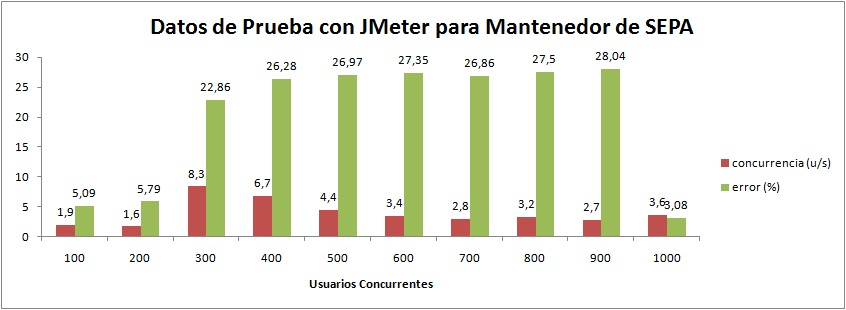
\includegraphics[scale=0.6,angle=0]{images/g1.jpg}
\caption{Gráfico de Cantidad de Usuarios contra Porcentaje de error y Concurrencia}

\end{center}
\end{figure}

\section{Recomendaciones}

Las 2 recomendaciones principales es que el sistema puede aguantar un poco más de lo que las pruebas de carga y estres puedan decirnos, ya que el ambiente en donde se trabaja tiene ciertas limitantes, por ejemplo el servidor de consulta es uno de prueba en el cual hay una cantidad limite de usuarios.

Para finalizar es necesario también aclarar que las pruebas contemplan a usuarios que están realizando exactamente la misma acción, lo que hace que el sistema se sobrecargue en ciertos aspectos como consultas a bases de datos de manera repetitiva. Dando a entender que esta no es una situación para nada real y altamente fuerte para el sistema y que en condiciones reales es muy probable que se comporte un poco mejor que lo que pueden decir los resultados.

\chapter{Diagrama del Proyecto}
\section{Información}
Esto es un servicio que alimenta a sus datos gracias a un servicio web, Usando el framework Apache CXF nos permite gestionar estos datos y nosotros con java y Spring Data somos capaces de entregárselos a nuestra base de datos PostgresSQL. De esta manera nosotros podemos con Spring Security ocupar los Beans de Spring que nos gestionan las paginas del sitio de mantenedores. El sitio por su parte esta echo con JSF para mostrar en pantalla sus datos, por encima tenemos un componente que enriquece las características de JSF llamado Primefaces, el cual nos agrega funcionalidad y características nuevas, como por ejemplo cajas de texto con parámetros que verifican los datos buscando errores en ellos así evitando completamente que el usuario use de mala manera el sitio.

Esto es un servicio que alimenta a sus datos gracias a un servicio web, Apache CXF nos permite gestionar estos datos y nosotros con java y Spring Data somos capaces de entregárselos a nuestra base de datos PostgresSQL. De esta manera nosotros podemos con Spring Security ocupar los Beans de Spring que nos gestionan las paginas del sitio de mantenedores. El sitio por su parte esta echo con JSF para mostrar en pantalla sus datos, por encima tenemos un componente que enriquece las características de JSF llamado Primefaces, el cual nos agrega funcionalidad y características nuevas, como por ejemplo cajas de texto con parámetros que verifican los datos buscando errores en ellos así evitando completamente que el usuario pueda mal usar el sitio.

\begin{figure}[!hbp]
\begin{center}
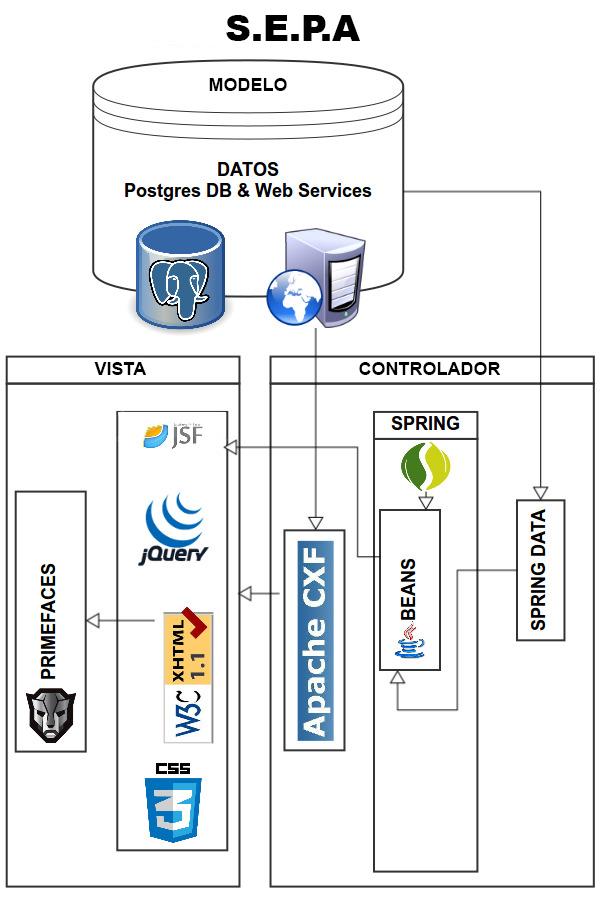
\includegraphics[scale=0.6,angle=0]{images/diagrama.jpg}
\caption{Diagrama general del sistema}

\end{center}
\end{figure}
\chapter{Evaluación de Costos}
\section{Puntos de Función}
Para evaluar los costos monetarios de este proyecto se utilizara el calculo de Puntos de Función para llegar a un valor justificado. Mediante una función matemática que utiliza varios parámetros, divididos en 2 ramas.

\section{Conteo de puntos}

\begin{enumerate}
	\item Ficheros Internos Lógicos (FIL): La información de los datos internos, contenida en bases de datos y ficheros de configuración.
	\item Ficheros Externos de Interfaz (FEI): El proyecto utiliza datos que son administrados por la aplicación DirDoc.
	\item Entrada Externa (EE): El sistema consume servicios web provenientes de otros sistemas.
	\item Salida Externa (SE): El sistema muestra la totalidad de los datos internos en su parte visual.
	\item Consulta Externa (CE): El sistema tiene mantenedores de todos sus datos, para poder ser modificables por los usuarios.
\end{enumerate}

\textbf{Tabla de valores ponderados}\\
\begin{tabular}{| l | l | l | l |}
\hline
\textbf{Característica} & \textbf{Ponderación} & \textbf{Valor} & \textbf{Resultado} \\
\hline
FIL & 25 & medio & 4\\
\hline
FEI & 25 & medio & 4\\
\hline
EE & 16  & alto  & 2\\
\hline
SE & 26  & alto  & 3\\
\hline
CE & 26  & alto  & 3\\
\hline
\end{tabular}
\\\\\\
\textbf{Tabla de valores calculados}\\
\begin{tabular}{| l | l | l | l | l |}
\hline
\textbf{TIPO} & \textbf{Bajo} & \textbf{Medio} & \textbf{Alto} & \textbf{Total} \\
\hline
EE & x3  & 4x4  & x6 & 16\\
\hline
SE & x4  & 4x5  & x7 & 20\\
\hline
CE & x3  & x4  & 2x6 & 12\\
\hline
FIL & x7 & x10 & 3x15 & 45\\
\hline
FEI & x5 & x7 & 3x10 & 30\\
\hline
TOTAL &  &  & & 123\\
\hline
\end{tabular}
\\\\\\
El total obtenido debe ser reparado con una serie de factores que se incluyen a continuación.

\section{Características Generales del Sistema}

En esta sección se evalúa con un número de 0 a 5 las distintas características que este sistema puede o no tener, y finalmente se ponderan para generar un valor que nos permite hacer el ajuste para el conteo de puntos anterior.

\begin{enumerate}
	\item Comunicación de Datos: [4 puntos] Varios teleprocesos pero con el mismo protocolo de comunicaciones.
	\item Proceso Distribuido: [4 puntos] Proceso de datos distribuidos y transferencia de datos en línea en ambas direcciones. Por ejemplo una red de cajeros automáticos en donde estos procesan parte de la transacción.
	\item Objetivos de Rendimiento: [4 puntos] Se utilizan herramientas de análisis de rendimiento durante el diseño, desarrollo e instalación, con el objetivo de alcanzar el rendimiento demandado por el usuario.
	\item Configuración de Explotación Usada intensamente por Otros Sistemas: [1 punto] Existen restricciones, pero son las usuales de cualquier equipo departamental. No es necesario hacer consideraciones especiales.
	\item Tasa de Transacciones: [2 puntos] Se prevén peaks de operaciones semanales.
	\item Entrada de datos EN-LÍNEA: [5 puntos] La entrada de datos interactivas superan el 30 por ciento de las transacciones.
	\item Eficiencia con el Usuario Final: [3 puntos] Seis o más factores, pero sin especiales requerimientos de eficiencia.
	\item Actualizaciones EN-LÍNEA: [4 puntos] Protección ante pérdidas y el sistema se ha de diseñar e implementar con estas consideraciones.
	\item Lógica de Proceso Interno Compleja: [5 puntos] La aplicación llevará incorporados sistemas de seguridad y control.
	\item Reusabilidad del Código: [5 puntos] La aplicación ha sido específicamente empaquetada y/o documentada para ser fácil de reutilizar.
	\item Contempla la Conversión y Facilidad de Instalación: [0 puntos] No reemplazamos un sistema existente o no se requiere conversión. Tampoco se enuncia nada sobre la instalación.
	\item Facilidad de Operación: [5 puntos] Sistema automático sin intervención.
humana
	\item Instalaciones Múltiples: [3 puntos] La aplicación correrá en múltiples entornos de Hw o Sw y se tiene en cuenta desde la fase de diseño.
	\item Facilidad de Cambios: [3 puntos] El cambio de la configuración se hace interactivamente y tiene efecto inmediato.
\end{enumerate}

\textbf{Cálculo de los puntos de función ajustados}\\
\begin{tabular}{| l | l | l |}
\hline
\textbf{No.} & \textbf{Factor de Complejidad} & \textbf{Valor}\\
\hline
1 &  Comunicación de Datos & 4 \\
\hline
2 &  Proceso Distribuído &4  \\
\hline
3 & Objetivos de Rendimiento  &4  \\
\hline
4 & Configuración Explotación Compartida  & 1 \\
\hline
5 & Tasa de Transacciones  & 2 \\
\hline
6 &  Entrada de Datos EN-LÍNEA &  5\\
\hline
7 & Eficiencia con el Usuario Final  &  3\\
\hline
8 & Actualizaciones En-LÍNEA  & 4 \\
\hline
9 & Lógica del Proceso Interno Compleja  &  5\\
\hline
10 & Reusabilidad del Código  &  5\\
\hline
11&  Contempla la Conversión e Instalación &  0\\
\hline
12& Facilidad de Operación  &  5\\
\hline
13& Instalaciones Múltiples  &  3\\
\hline
14& Facilidad de Cambios  & 3 \\
\hline
\multicolumn{2}{|c|}{Factor de Complejidad Total (FCT)} & 48\\
\hline
\end{tabular}
\\\\\\

\section{Puntos de función ajustados}
La siguiente formula describe la cantidad ajustada de puntos de función y estos a su ves son multiplicados por el valor en horas de lo que cuesta en tiempo y dinero, cada uno de los puntos. Obteniendo finalmente el valor ponderado del proyecto en si.

\begin{math}
PFA=PFSA * ( 0.65 + ( 0.01 * FCT ) = 123 * ( 0.65 + ( 0.01 * 48 ) = 139
\end{math}

\begin{math}
139 * (Horas * Valor Hora) = 139 * (4 * 4000) = 2224000
\end{math}

El proyecto vale un mínimo de 2.224.000 pesos.

\chapter{Corolario}

\section{Garantías de calidad}

La calidad de este sistema se ve potenciada por varios aspectos, los cuales se explicaran a continuación:

\begin{enumerate}
	\item Uso de Metodología de Trabajo: El uso de PSP fortalece el desempeño del proyecto, mostrando los errores que el proceso de desarrollo pueda mostrar, desde esta perspectiva es necesario destacar que cuando se van anotando los errores estos tienden a disminuir con el tiempo por lo que en las etapas finales es muy difícil encontrar errores en el desarrollo.
	\item Uso de Patrón de diseño: El patrón MVC ha echo de este proyecto un ente robusto y fuerte que puede ser mejorable incluso con poco conocimiento, ya que posee una base solida que sustenta su funcionamiento, por lo cual los cambios que se puedan nesesitar en el futuro harán uso de las herramientas que se fabricaron el desarrollo mismo.
	\item Uso de Java y Frameworks: Esto nos permite una autonomía en varios aspectos, ya que nosotros como impulsores de proyectos tenemos siempre que velar por que todo el desarrollo sea altamente eficiente, y una manera muy clara de obtener eso es mediante del uso de herramientas que ya han sido muy probadas y se encuentran en uso de muchos otros proyectos. Dado que en otros sistemas esto ha funcionado muy bien es de esperar que en el nuestro también funcione excelente.
	\item Pruebas de rendimiento: Las pruebas sobrecargan el sistema de tal manera que nosotros podemos decir a ciencia cierta que el software es capaz de resistir lo que los datos nos entregan, y eso nos demuestra que el trabajo realizado cumple con ciertas características que hacen a un proyecto web por lo menos algo que gran valor.
\end{enumerate}

Finalmente con de estos puntos se puede tener una clara idea de la calidad del producto que se entrega y de como este puede ir mejorando todavía, e inclusive puede cambiar y adecuase a otras necesidades.

\section{Conclusión}
El trabajo correspondiente al Sistema Mantenedor e Integrador en SEPA ha mostrado una forma de como recuperar datos que pueden ser difíciles de manejar. Los datos para este trabajo no estaban del todo bien organizados, esto quiere decir que cuando uno observa los datos, es posible encontrar insuficiencias de campos en los objetos mostrados en las tablas de los mantenedores, para lo cual los Mantenedores están preparados para ingresar datos en los sectores que lo requieran.

También es posible identificar errores estructurales de información. En el sistema Integrador entraban datos que contenían errores repetidos en todas las filas de ciertas tablas, para lo cual este sistema esta preparado para resistir ese tipo de datos y cargar una data estándar que mas adelante será reparada por el sistema Mantenedor.

Finalmente como análisis final se determina que este trabajo es necesario para cada organización educacional chilena, ya que en cada una de ellas existen datos que tienen estructuras antiguas de orden e indexado, lo que hace difícil para sistemas nuevos o venideros generar productos que ayuden en el desempeño de actividades, tales como organización económica de la institución académica, orden y mantenimiento de los sistemas docentes.
\section{Trabajo Futuro}
Para ampliar las posibilidades de un trabajo que descansa sobre el valor de potenciar las capacidades administrativas de una institución académica, es necesario hacer estudios que posibiliten un mayor alcance de datos, tal como lo hace sepa, por tal razón es de vital importancia promover nuevas mejoras que hagan de este sistema una herramienta completa en el desarrollo de las capacidades generales de una organización, como lo es la Universidad Tecnológica Metropolitana.

Finalizando, se puede pensar que un trabajo como este es perfectamente capaz de entregar datos y argumentos solidos en pos de generar estudios científicos relacionados con indicadores de calidad en educación, puesto que con el sistema SEPA en las condiciones actuales, se tienen todas las herramientas preparadas para tales propósitos. 
\bibliographystyle{plain}
\bibliography{bibliografia.bib}
\end{document}